\section{Evaluation}
\label{sec:evaluation}
In this section we present results regarding the ability of VaRTOS to maximize utility by modification of task knob values as well as the corresponding error in energy consumption vs. the specified energy budget.  Finally, we evaluate the VaRTOS architecture in terms of both energy and memory overheads.  

\subsection{Minimizing Energy Consumption Error}

\begin{figure*}
\centering
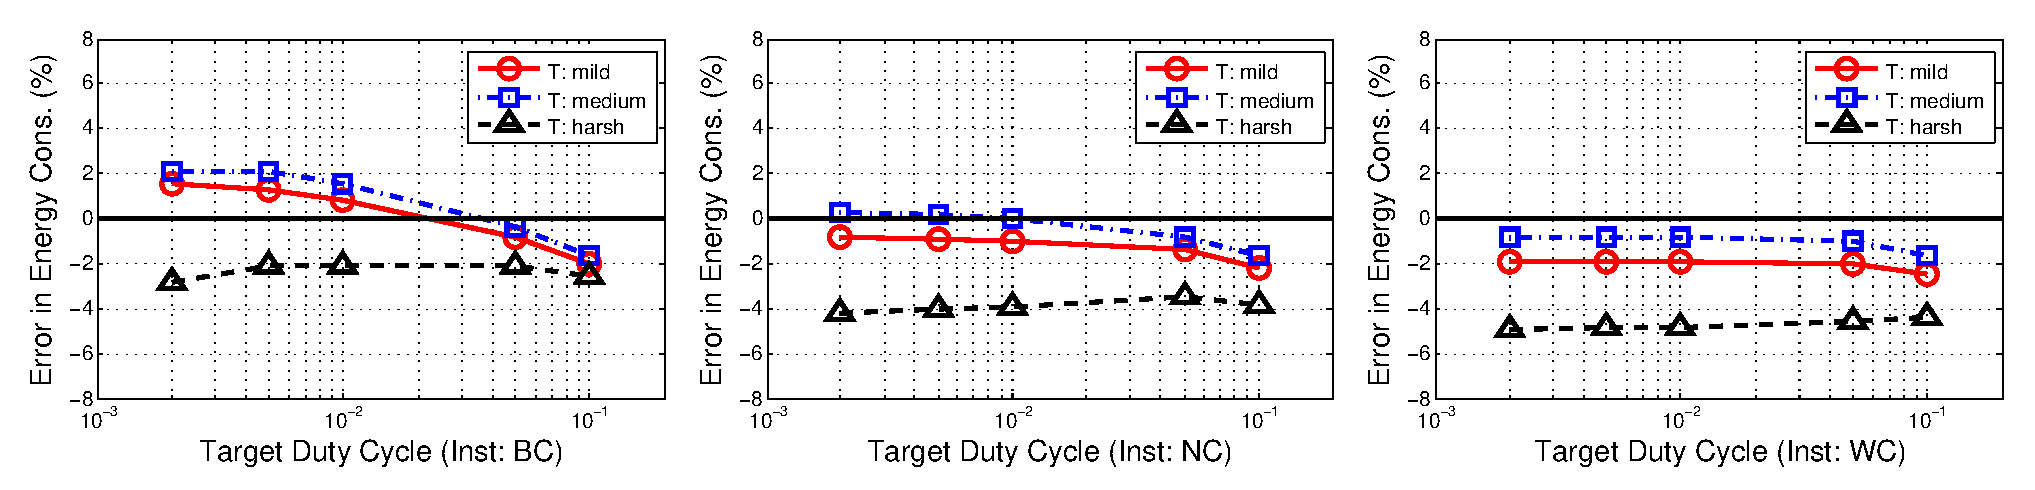
\includegraphics[width=1\textwidth]{figures/app1_nonoise}
\caption{\label{fig:app1_dc}Error in energy consumption for various optimal duty cycles and for mild, medium, and harsh environments.  From left to right, figures represent the best case, nominal case, and worst case power instances in 45 nm.}
\end{figure*}

%\begin{figure*}
%\centering
%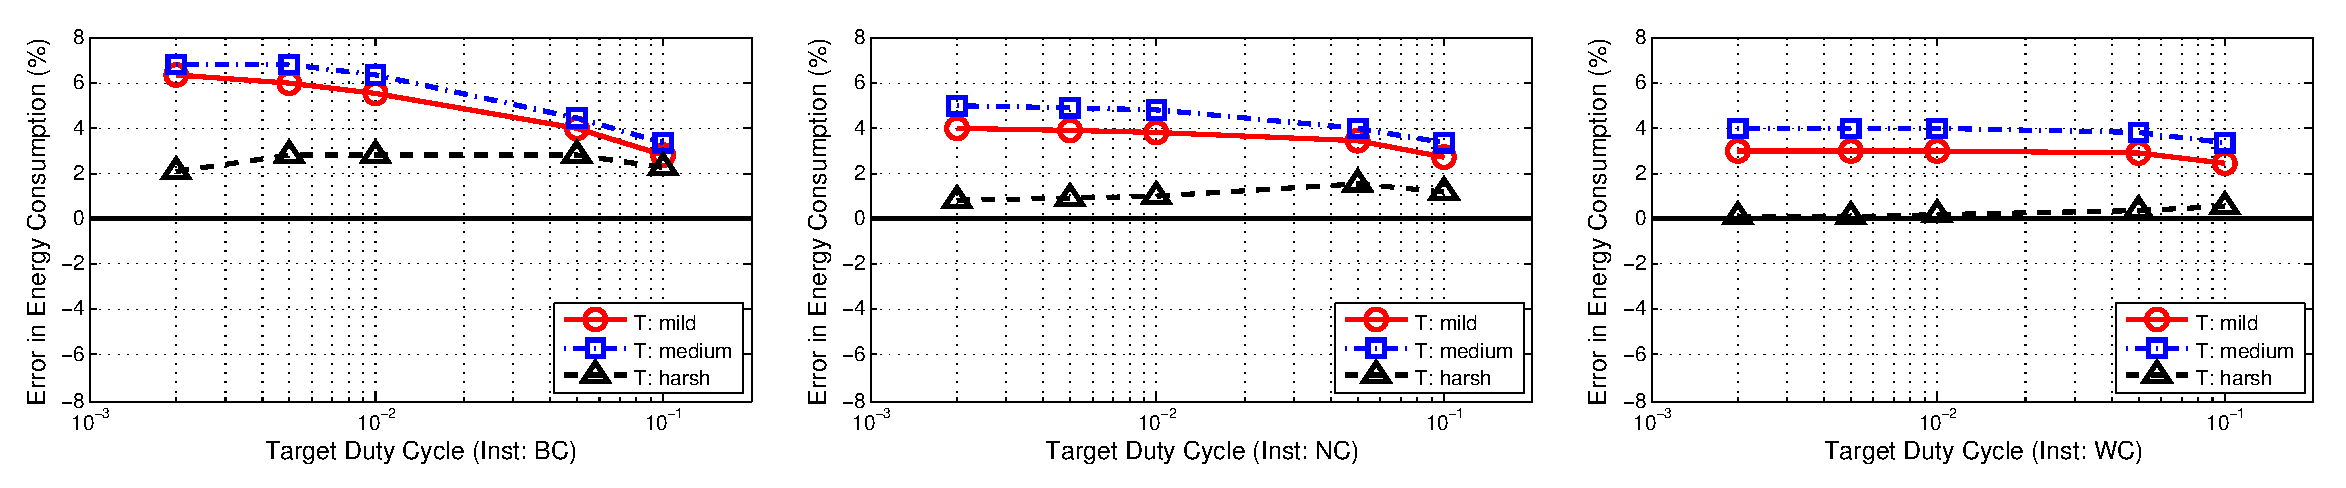
\includegraphics[width=1\textwidth]{figures/app1_guardband.eps}
%\caption{\label{fig:app1_dc_guardband}App 1 results, no noise}
%\end{figure*}

In order to achieve accurate energy consumption to meet a lifetime goal, VaRTOS needs to accurately be able to achieve the overall system duty cycle $d_{sys}^*$.  To test this, we constructed a simple application with only a single task containing a knob with fine granularity values.  Then, using the tool shown in Figure \ref{fig:gui}, we specified various values for $E$ and $L$ that would ideally lead to a particular $d_{sys}^*$ for each of the power instance models (best-, nominal-, and worst-case) as well as three temperature profile instances (harsh, medium, and mild).  The target duty cycles were $d_{sys}^* \in \{0.002, 0.005, 0.01, 0.05, 0.1\}$, or from 0.2\% up to 10\%, and the resulting errors in energy consumption are shown in Figure \ref{fig:app1_dc}.  Note that errors are larger in harsher environments, where any errors in the power models will be magnified.  In the worst case, an error of 4.9\% in energy consumption is seen for a harsh environment and for the worst-case power instance (far right plot in Figure \ref{fig:app1_dc}). This means that, in the worst case, a 5\% guard band in lifetime or in energy is necessary if the lifetime goal is to be treated as a hard constraint. 

To give more intuition into what this error in energy consumption means, we compared energy consumption for tasks running in VaRTOS (modeling power on a per-instance basis) with those assuming `worst-case' power consumption.  True worst-case power consumption is difficult to define, due to the long tail distribution for power across temperature.  Because of this, we define worst-case power as the average power consumption for the worst-case instance from Section \ref{sec:methods} across the temperature range $[0^\circ C,~45^\circ C]$, particularly $P_s = 330 ~\mu$W and $P_a = 1.187$ mW.  Figure \ref{fig:app1_energy} shows the disparity between the two.  Without per-instance power modeling, energy consumption is in some cases over 70\% off, and in only one case is it below 10\% error.  With per-instance power modeling using VaRTOS, the error has dropped to below 2\% in most cases and around 5\% in the worst case. Note that a positive percent error means a surplus in energy after the lifetime has been met while a negative means an energy deficit (and likewise a premature death).  Energy errors are mostly positive here because of the worst-case power assumption. 

Similarly, Figure \ref{fig:app1_dc2} shows the cause of this energy error disparity---the duty cycle ratio remains constant if worst-case power is assumed while it is allowed to vary when instance-specific power modeling is introduced.  This will translate into an increase in the quality of service for a particular application (e.g. more data collected, a higher communication rate) by using what would have been surplus energy. 

\begin{figure*}[t]
\centering
{\centering
\begin{minipage}{0.47\textwidth}
  \centering
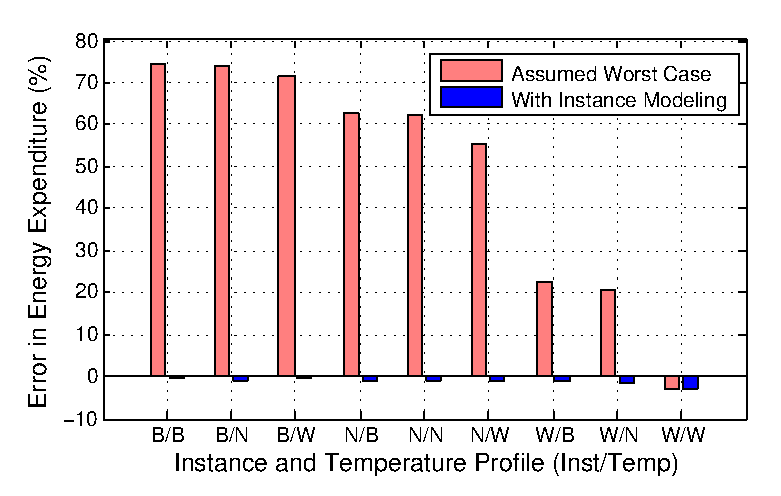
\includegraphics[width=\textwidth]{figures/app1_energycomp}
  \captionof{figure}{\label{fig:app1_energy}Errors in energy consumption for a single-task application for worst-case power assumptions and per-instance power modeling.}
\end{minipage}
\hspace{.04\textwidth}
\begin{minipage}{0.47\textwidth}
  \centering
\includegraphics[width=\textwidth]{figures/app1_dutycycles}
  \captionof{figure}{\label{fig:app1_dc2}Average duty cycles of a single-task application for worst-case power assumptions and per-instance power modeling. }
\end{minipage}
}
\end{figure*}



\begin{figure}
\centering
\includegraphics[width=0.47\textwidth]{figures/app1_oracle}
\caption{\label{fig:app1_oracle}Total utility, $u_{sys}$, for VaRTOS vs. the oracle system.}
\end{figure}

\subsection{Utility and Oracle Comparison}
The results in the previous section showed that VaRTOS is able to meet a given energy budget with low error, resulting in an accurate system lifetime.  In Section \ref{sec:optimization} we argued that spending would-be surplus energy will increase system utility.  In this section, we substantiate this claim by comparing the utility of the single task app running in VaRTOS to that of an all-knowledgeable oracle system.  Unlike the true VaRTOS system, the oracle system is allowed the following privileges: (1) complete knowledge of the temperature profile for the test year; (2) perfect knowledge of task behavior (i.e. $\mathcal{K}_i$); (3) full accuracy models for $P_s$ and $P_a$; and (4) zero overhead for optimization routines.  Figure \ref{fig:app1_oracle} shows the utilities for both the oracle and VaRTOS.  In most cases VaRTOS achieves within 10\% of the oracle utility, and is as much as 20\% off in the worst case.  Note that this comparison is specific to the construction of utility $u_i$ as defined in Equation \ref{eq:util}, and other utility curves may cause variations in this metric.


\subsection{Energy and Memory Overhead}
Energy consumption by the various VaRTOS subsystems must be minimized in order to prevent worsening the very thing we are trying to correct.  Similarly, the memory required for VaRTOS must be kept reasonably low in order to make it a viable option for resource-constrained platforms.  \\

\noindent\emph{\underline{Memory Overhead:}}
The amount of program memory (.text, .data) and volatile memory required for VaRTOS depends on the application that the developer is designing.  As a baseline, VaRTOS requires a modest increase in the `.text' section over the vanilla FreeRTOS framework from 2.29 kB to 6.80 kB ( a 4.51 kB increase).  This includes a lightweight library for math functions required for optimization routines (including exponential, logarithmic, and square root functions) as well as a preemptive scheduler.  If a full math library needs to be used for the application itself, these functions can be replaced and the overhead amortized.  In terms of volatile memory, an additional 508 bytes baseline is required (480  bytes of this is due to the power learning procedure and, if the developer is so motivated, can be reused after the models have converged).  An additional 46 bytes per task is also required for knob modeling and other parameters.  Finally, the temperature profile is stored in program ROM as a constant array and consumes only 10 additional bytes. \\

%
%memory: 40 floats for Ps, Pa, temp: 120 floats for power convergence, can be freed if memory management available. float for (psslope, psoffset, paslope, paoffset, optimaldc). int for (lifetime, energy). 
%
%added memory per task: int for knob, kmin, kmax, float for pi, float for time model times (4), float for Koffset and Kslope and dcopt. also (4) for knobs in the array 
%

\noindent\emph{\underline{Energy Overhead:}}
The largest energy overhead in VaRTOS comes from the scheduler itself, which, if context swaps occur every 10 ms, causes a baseline system duty cycle of 0.1\%. This ratio can be decreased if coarser granularity context swaps are acceptable.  The power consumption attributed to this 0.1\% depends on the power consumption of the processor and the environmental temperature, but in the worst case it consumes $P_{os} = 0.001\cdot(1.187~mW) + 0.999\cdot(330~\mu W) = 331~\mu W \approx P_s$. In other words, the sheduler adds only marginal power consumption on top of the baseline sleep power. 

Other potential energy consuming processes attributed to VaRTOS include knob modeling, power measurement and fitting, finding the optimal $d_{sys}^*$, and finding the optimal knob values.  The amount of processing time spent in these tasks is negligible:  reading power and temperature takes 250 $\mu$s and occurs only 40 times over the course of a deployment (10 ms total); knob perturbations take 48 $\mu$ s and occur 4$\cdot N$ times (for $N$ tasks); performing a 40-point linear regression (for power curves and as an upper bound for modeling $\mathcal{K}_i$) takes 40 ms and occurs twice ($P_s$ and $P_a$) per deployment and once per task; finding $d_{sys}^*$ takes 54 ms and occurs once unless tasks are deleted and created after the initial optimization; and finally finding optimal $d_i^*$ and $k_i^*$ values takes 345 $\mu$s.  In total, these added tasks consume less than 1 mJ in the worst-case for a 1 year deployment, a negligible overhead if our energy budget is 12960 Joules (2 AAA batteries) as in the following section. Note, however, that (1) taking power and temperature measurements is likely to consume additional power for analog to digital conversions and (2) a more difficult calculation in energy overhead comes from the result of perturbing knob values in the modeling phase for $\mathcal{K}_i$.  The latter depends on the nature and number of tasks, as well as the length of $t_{super}$. 



















